\section{Исследование и построение решения задачи}
\label{sec:Chapter4} \index{Chapter4}

Исходя из требований, поставленных ранее, данным условиям соответствуют состязательные генеративные модели. Во-первых, они хорошо работают с данными большой размерности, достигая передовые результаты в задачах генерации изображений \cite{style-gan}, а во-вторых, генерация данных заключается в отображении элементов скрытого пространства в пространства данных, вызовом генератора, то есть за один шаг.

Для того чтобы связать состязательные генеративные модели с задачей мостов Шрёдингера, необходимо подробнее рассмотреть свойства и особенности GAN.

\subsection{Состязательные генеративные модели (Generative-adversarial networks, GAN) и их обобщение f-GAN}
В статье Гудфеллоу \cite{gan} был представлен новый метод оценки генеративных моделей с использованием состязательного обучения.

Такой метод обучает генеративную модель $G$ состязательно , вводя дискриминативную модель $D$, которая пытается определить, является ли выборка реальной или сгенерированной:
\begin{multline*}
    \min_{G}\max_{D}V(G, D) = \min_{G}\max_{D} \mathbb{E}_{x\sim p_{data}} [\log D(x)] - \mathbb{E}_{x\sim p_g} [1 - \log D(x)] = \\ = \min_{G}\max_{D} \mathbb{E}_{x\sim p_{data}} [\log D(x)] - \mathbb{E}_{z\sim p(z)} [1 - \log D(G(z))].
\end{multline*}

Важно отметить, что авторы доказывают, что выбрав оптимальный дискриминатор $D^*$, мнинимизационная задача аналогична минимизации дивергенции Йенсена-Шеннона между $p_{data}$ и $p_g$, то есть:
\begin{multline}
    \min_{G}\max_{D} \mathbb{E}_{x\sim p_{data}} [\log D(x)] - \mathbb{E}_{x\sim p_g} [1 - \log D(x)] = \\ 
    = \min_{G} \mathbb{E}_{x\sim p_{data}} [\log D^*(x)] - \mathbb{E}_{x\sim p_g} [1 - \log D^*(x)] = \min_{G}D_{JS}(p_{data}||p_g) - 2\log 2.
    \label{eq:gan}
\end{multline}

Опираясь на этот факт, в статье \cite{fgan} расширяется теория состязательных сетей до более общего принципа, используя вариационное (двойственное) представление f-дивергенции.

Для понимания введем понятие \textit{сопряженной функции}.
\begin{definition}[Сопряженная функция]
    Пусть $f:dom(f) \rightarrow \mathbb{R}$ -- выпуклая функция, где $dom(f) \subseteq \mathbb{R}$ -- это интервал. Тогда выпуклая сопряженная функция $f$ — это функция $f: dom(f^*) \rightarrow \mathbb{R}$ определенная следующим образом:
    \begin{equation*}
        f^*(y) = \sup_{x\in dom(f)}(yx - f(x)),
    \end{equation*}
    где $dom(f^*):=\{y \in \mathbb{R}: f^*(y) < \infty\}$.
\end{definition}

Для формулировки вариационного представления также потребуются свойства выпуклой сопряженной функции.
\begin{property}
    Выпуклая сопряженная функция $f^*$ функции $f$ удовлетворяет следующим свойствам:
    \begin{enumerate}
        \item $f^*$ непрерывна в своей области определения;
        \item $f^*$ выпукла;
        \item $(f^*)^* = f$.
    \end{enumerate}
\end{property}

Теперь, можно сформулировать теорему двойственности.
\begin{theorem}[Вариационное (двойственное) представление f-дивергенции]
    Для любой f-дивергенции, имеется:
    \begin{equation}
        D_f(P||Q) = \sup_{g:\mathcal{X} \rightarrow \mathbb{R}} \mathbb{E}_P[g(X)] - \mathbb{E}_Q[f^*(g(X))],
        \label{eq:dual}
    \end{equation}
    где $f^*$ -- выпуклая сопряженная функция функции $f$, а супремум берется по всем функциям $g$, у которых оба математических ожидания конечны.
\end{theorem}

\begin{proof}
    \begin{equation*}
        D_f(P||Q) = \int_\mathcal{X} f\left(\frac{dP}{dQ}(x)\right))dQ(x) = \int_\mathcal{X} \sup_{y \in dom(f^*)}\left(y\frac{dP}{dQ}(x) - f^*(y)\right)dQ(x)
    \end{equation*}
    
    Теперь вместо того, чтобы брать супремум по $y$, мы можем заменить $y$ супремумом по некоторой функции $g:\mathcal{X} \rightarrow \mathbb{R}$, поскольку $y$ обычно зависит от $x$. Затем применяя неравенство Йенсена:
    \begin{multline*}
        D_f(P||Q) \geq \sup_{g:\mathcal{X} \rightarrow \mathbb{R}} \left(\int_\mathcal{X}g(x)dP(x) - \int_{\mathcal{X}}f^*(g(x))dQ(x)\right) = \\ = \sup_{g:\mathcal{X} \rightarrow \mathbb{R}} \left(\mathbb{E}_{x\sim P}[g(x)] - \mathbb{E}_{x\sim Q}[f^*(g(x))]\right).
    \end{multline*}
    
    Вышеуказанная нижняя граница является жесткой и достигается при $g(x) = f'\left(\frac{dP}{dQ}(x)\right)$
\end{proof}

\begin{table}[h]
    \centering
    \begin{tabular}{||c|c|c|c||}
    \hline
    \textbf{Дивергенция} & \textbf{$g_f$} & \textbf{$dom_{f^*}$} & \textbf{$f^*(x)$} \\ \hline \hline
    Кульбака—Лейблера (КЛ) & $x$ & $\mathbb{R}$ & $\exp(x - 1)$ \\ \hline
    Обратная КЛ & $-\exp(-x)$ & $\mathbb{R}_{-}$ & $-1 - \log(-x)$ \\ \hline
    $\chi^{2}$ Пирсона & $x$ & $\mathbb{R}$ & $\frac{1}{4}x^2 + x$ \\ \hline
    Хеллингера & $1 - \exp(-x)$ & $x < 1$ & $\frac{x}{1 - x}$ \\ \hline
    Йенсена-Шеннона & $\log(2) - \log(1 + \exp(-x))$ & $x < \log(2)$ & $-\log(2 - \exp(x))$ \\ \hline
    GAN & $-\log(1 + \exp(-x))$ & $\mathbb{R}_{-}$ & $-\log(1 - \exp(x))$ \\ \hline
    \end{tabular}
    \caption{Рекомендуемые функции активации последнего слоя и сопряженные функции для различных f-дивергенций.}
    \label{tab:var-div}
\end{table}

Таким образом авторы \cite{fgan} формулируют следующую целевую функцию:
\begin{equation}
    F(G, D) = \mathbb{E}_{x\sim p_{data}} \left[ g_f (D(x)) \right] + \mathbb{E}_{z\sim p(z)} \left[ -f^* (g_f (D(G(z)))) \right],
    \label{eq:f-gan}
\end{equation}
где $G$ и $D$ -- генератор и дискриминатор, аналогично GAN, а $g_f$ -- функция активации, которая ограничивает выход дискриминатора на область определения функции $f^*$.

Так, например, выбирая $f^*(x) = - \log(1 - \exp(x))$ и $g(x) = \log \frac{p(x)}{p(x)+q(x)}$ выводится целевая функция состязательных сетей \ref{eq:gan}. Примеры остальных дивергенций приведены в таблице \ref{tab:var-div}.

Также авторы упростили процедуру оптимизации седловой точки, которая изначально была введена в GAN и вывели целевые функции для всех f-дивергенций, самое важное, в с число,которых входит и дивергенция Кульбака-Лейблера, применяющаяся в задаче мостов Шрёдинегера.

\subsection{Состязательные мосты Шрёдингера}
Вдохновившись идеей представления дивергенций в вариационном виде, в данной работе предлагается формулировка минимизационной задачу мостов Шрёдингера аналогичным способом. Для этого рассмотрим статическую постановку задачи мостов Шрёдингера \ref{static}. 

Чтобы представить совместные распределения в алгоритме IPF (алгоритм \ref{alg:ipfp}) с помощью двойственного представления f-дивергенций (задача \ref{eq:dual}), вариационное представление рассматривается с учетом измеримого пространства $(\mathcal{X}\times\mathcal{Y}, \Sigma)$ вместо $(\mathcal {X}, \Sigma)$. Таким образом, дивергенции в шагах алгоритма IPF (алгоритм \ref{alg:ipfp}) будут иметь следующий вид:

\begin{equation}
    \begin{split}
        D_{KL}(p(x,y)||q^*_{i-1}(x,y)) = \max_{g:\mathcal{X}\times\mathcal{Y} \rightarrow \mathbb{R}} \mathbb{E}_{p(x,y)}[g(x,y)] - \mathbb{E}_{q^*_{i-1}(x,y)}\left[e^{(g(x,y) - 1)}\right], \\
        D_{KL}(q(x,y)||p^*_{i}(x,y)) = \max_{v:\mathcal{X}\times\mathcal{Y} \rightarrow \mathbb{R}} \mathbb{E}_{p^*_{i}(x,y)}[v(x,y)] - \mathbb{E}_{p^*_{i}(x,y)}\left[e^{(v(x,y) - 1)}\right],
    \end{split}
\end{equation}
обратный и прямой шаги, соответственно.

Аналогично f-GAN (уравнение \ref{eq:f-gan}) параметризуем вариационные функции $g$ и $v$ с помощью нейронных сетей $D$ и $T$, соответственно, и получаем следующие минимизационные задачи:
\begin{equation}
    \begin{split}
        \min_{p(x,y) \in \mathcal{D}(\cdot, \pi_T)}\max_{D}\mathbb{E}_{p(x,y)}[D(x,y)] - \mathbb{E}_{q^*_{i-1}(x,y)}\left[e^{(D(x,y) - 1)}\right], \\
        \min_{q(x,y) \in \mathcal{D}(\pi_0, \cdot)}\max_{T}\mathbb{E}_{q(x,y)}[T(x,y)] - \mathbb{E}_{p^*_{i}(x,y)}\left[e^{(T(x,y) - 1)}\right].
    \end{split}
\end{equation}

Благодаря вариационному представлению также возникает возможность избавиться от ограничений в минимизационной задаче, а именно следующих: $p(x,y) \in \mathcal{D}(\cdot, \pi_T)$ и $q(x,y) \in \mathcal{D}(\pi_0, \cdot)$. Для этого совместные распределения $p(x,y)$ и $q(x,y)$ представляются через условное и маргинальное распределения. Таким образом, целевая функция примет следующий вид:

\begin{equation}
    \begin{split}
        \min_{p(x|y)}\max_{D}\mathbb{E}_{\pi_T(y)}\mathbb{E}_{p(x|y)}[D(x,y)] - \mathbb{E}_{\pi_0(x)}\mathbb{E}_{q^*_{i-1}(y|x)}\left[e^{(D(x,y) - 1)}\right], \\
        \min_{q(y|x)}\max_{T}\mathbb{E}_{\pi_0(x)}\mathbb{E}_{q(y|x)}[T(x,y)] - \mathbb{E}_{\pi_T(y)}\mathbb{E}_{p^*_{i}(x|y)}\left[e^{(T(x,y) - 1)}\right].
    \end{split}
\end{equation}

Для того, чтобы параметризовать условное распределение, предлагается использовать аналогичные подход, предложенный в статье условного GAN \cite{cond-gan}, основная суть которого заключается в том, что процесс генерации идет из конкатенации шума и обуславливаемого объекта. Схема такой генеративной модели изображена на рисунке \ref{fig:cond-gan}.

\begin{figure}
    \centering
    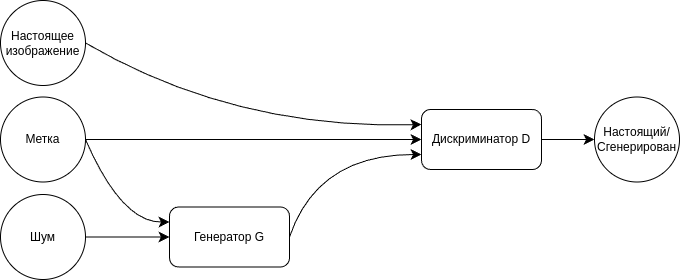
\includegraphics[width=0.75\linewidth]{images/cond_gan.png}
    \caption{Схема условного GAN}
    \label{fig:cond-gan}
\end{figure}

Применяя эту идею, получим следующие целевые функции:
\begin{equation}
    \begin{split}
        B(D, G) = \mathbb{E}_{\pi_T(y)}\mathbb{E}_{p(z)}[D(G(z, y),y)] - \mathbb{E}_{\pi_0(x)}\mathbb{E}_{p(z)}\left[e^{(D(x, K(z, x)) - 1)}\right], \\
        F(T, K) = \mathbb{E}_{\pi_0(x)}\mathbb{E}_{p(z)}[T(x, K(z, x))] - \mathbb{E}_{\pi_T(y)}\mathbb{E}_{p(z)}\left[e^{(T(G(z, y),y) - 1)}\right],
    \end{split}
    \label{eq:objective}
\end{equation}
где $G$ и $K$ -- генераторы, параметризованные нейронными сетями.

Для того, чтобы полноценно реализовать алгоритм IPF с помощью состязательного обучения необходимо проинициализировать $q^0(x|y)$ с помощью условного распределения $p^{\mathbb{W}^\gamma}(y|x) = \mathcal{N}(y| x, \gamma\mathbb{I})$. Для этого на первом шаге обратного прохода будем сэмплировать из заданного априорного распределения, то есть:
\begin{equation*}
    \mathbb{E}_{\pi_T(y)}\mathbb{E}_{p(z)}[D(G(z,y),y)] - \mathbb{E}_{\pi_0(x)}\mathbb{E}_{\mathcal{N}(y| x, \gamma\mathbb{I})}\left[e^{(D(x, y) - 1)}\right].
\end{equation*}
В итоге, получим новый состязательный алгоритм IPF (алгоритм \ref{alg:adv-ipf}).

\begin{algorithm}
\caption{Состязательный IPF}\label{alg:adv-ipf}
\KwInput{$\pi_0(x)$, $\pi_T(y)$, $p(y|x)$}
\KwOutput{$G^i, K^i$}
Инициализируем $i = 0$\;
\While{не сойдется}{
    $G^i = \arg\min_{G}\max_{D}B(D, G)$\;
    $K^i = \arg\min_{K}\max_{T}F(T, K)$\;
    $i:=i+1$\;
   }
\end{algorithm}

Предложенный метод удовлетворяет всем поставленным качествам. Во-первых, отображение происходит за один шаг, так как для того, чтобы отобразить данные из одного распределения в другое, необходимо использовать один раз $G$ или $K$. Во-вторых, в силу того, что метод наследует подход состязательного обучения, результирующая модель хорошо справляется с данными большой размерностью.

\newpage
